

\chapter{Diseño e implementación} % Main chapter title

\label{Chapter3} % Change X to a consecutive number; for referencing this chapter elsewhere, use \ref{ChapterX}



En este capítulo se presentan los detalles del diseño de los nodos sensores y actuadores que conforman el trabajo, como así también los de la implementación de la aplicación Thingsboard.

\section{Arquitectura de la solución}
\label{sec:Arquitectura de la solución}

%Como se observa en la figura \ref{fig:blockdiagram}, el invernadero inteligente está compuesto por un conjunto de subsistemas encargados de las diferentes funciones de medición y control de variables, una aplicación central y un sistema que permita el acceso remoto de forma segura.

Para la implementación del prototipo propuesto en el trabajo se requirió la construcción de diferentes subsistemas encargados de las múltiples funciones dentro del invernadero inteligente. En forma general, cada uno de estos módulos opera en forma independiente del resto y se comunican por medio de una red inalámbrica con una aplicación central. 

Para garantizar el acceso de los usuarios desde Internet se desarrolló una interfaz segura que no involucra costos al cliente y no requiere cambios de configuración en su red hogareña.

En la figura \ref{fig:blockdiagram} se observa la arquitectura diseñada con los subsistemas implementados.


\begin{figure}[h]
	\centering
	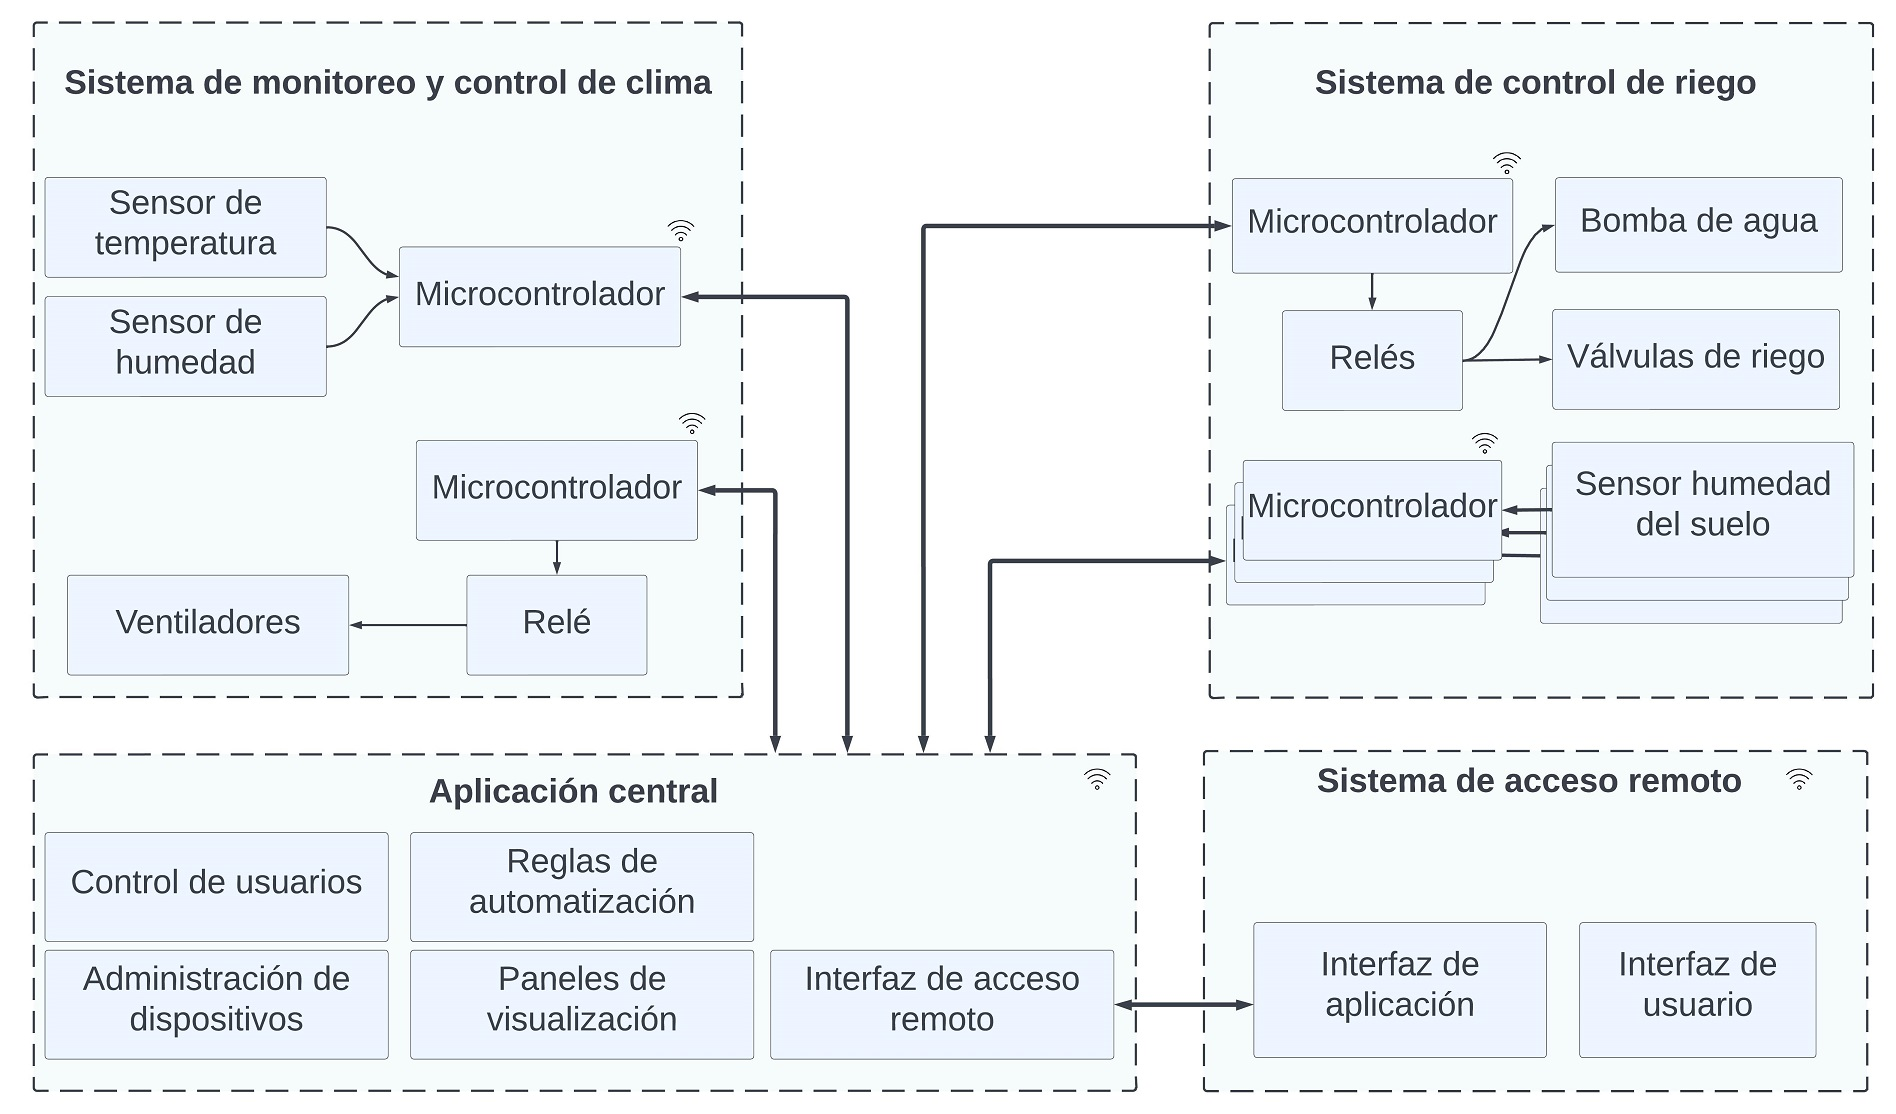
\includegraphics[width=1.0\textwidth]{./Figures/blockdiagram4.jpg}
	\caption[Arquitectura del sistema.]{Arquitectura del sistema.}
	\label{fig:blockdiagram}

\end{figure}

\subsection{Detalle de los sistemas}
\label{Detalle de los sistemas}

A continuación se detallan los subsistemas implementados en el trabajo:

\begin{itemize}
\item Sistema de monitoreo y control de clima: es responsable de medir la temperatura y humedad ambiente en el invernadero y enviar estas variables a la aplicación central. En base a los valores recibidos, la aplicación determina si es necesario enviar la señal de encender los ventiladores al microcontrolador correspondiente, y generar una alerta de aviso a los usuarios.


%
%\item Módulo de monitoreo de clima: es responsable de sensar la temperatura y humedad ambiente en el invernadero y enviar estas variables a la aplicación central para determinar las acciones a tomar en cuanto al control del clima.

\item Sistema de control de riego: está compuesto por múltiples sensores de humedad de suelo con sus respectivos microcontroladores que se distribuyen conforme a los circuitos de riego configurados. Los sensores proceden a enviar las mediciones a la aplicación central en donde se procesan los valores y en caso de ser necesario se dispara la señal de encendido a la válvula del circuito que corresponda, y luego a la bomba de agua para así comenzar el riego. Al mismo tiempo, el usuario recibe un alerta de accionamiento de la bomba.

\item Aplicación Central: constituye el cerebro del invernadero y es la encargada de almacenar los parámetros de configuración de los diversos sensores y actuadores, procesar los mensajes recibidos, disparar acciones y alertas y visualizar el estado general.

\item Sistema de acceso remoto: permite el acceso de usuarios a reportes del sistema en forma segura desde Internet.   
\end{itemize}

\subsection{Protocolos de comunicación}
\label{Protocolos de comunicación}
%\textit{Aquí se describe cómo se comunican los sistemas con la aplicación central y los protocolos usado en cada caso.}

%En la selección del software de la aplicación central se contempló la compatibilidad con múltiples protocolos de comunicación. Sin embargo limitaciones de configuración específicas, tal como el tiempo de retención de los mensajes en las colas de MQTT, forzaron el utilizar diferentes protocolos dependiendo del módulo en cuestión. Otro factor condicionante, como se detalla en la sección \ref{sec:Ciberseguridad del sistema}, fue el carecer de una CA que emita certificados que todos los componentes puedan confiar.

En esta sección se describe cómo se comunican los sistemas con la aplicación central y los protocolos usado en cada caso.

Si bien tanto los módulos de hardware como el software soportan una gran variedad de protocolos, basados en los requerimientos del proyecto, se buscó implementar MQTT.

%la implementación final estuvo dada por los requerimientos especificos y/o limitaciones de los sistemas.

En la figura \ref{fig:blockprotos} se ilustran los diferentes protocolos usados y en la tabla los diferentes usos. 

\begin{figure}[h]
	\centering
	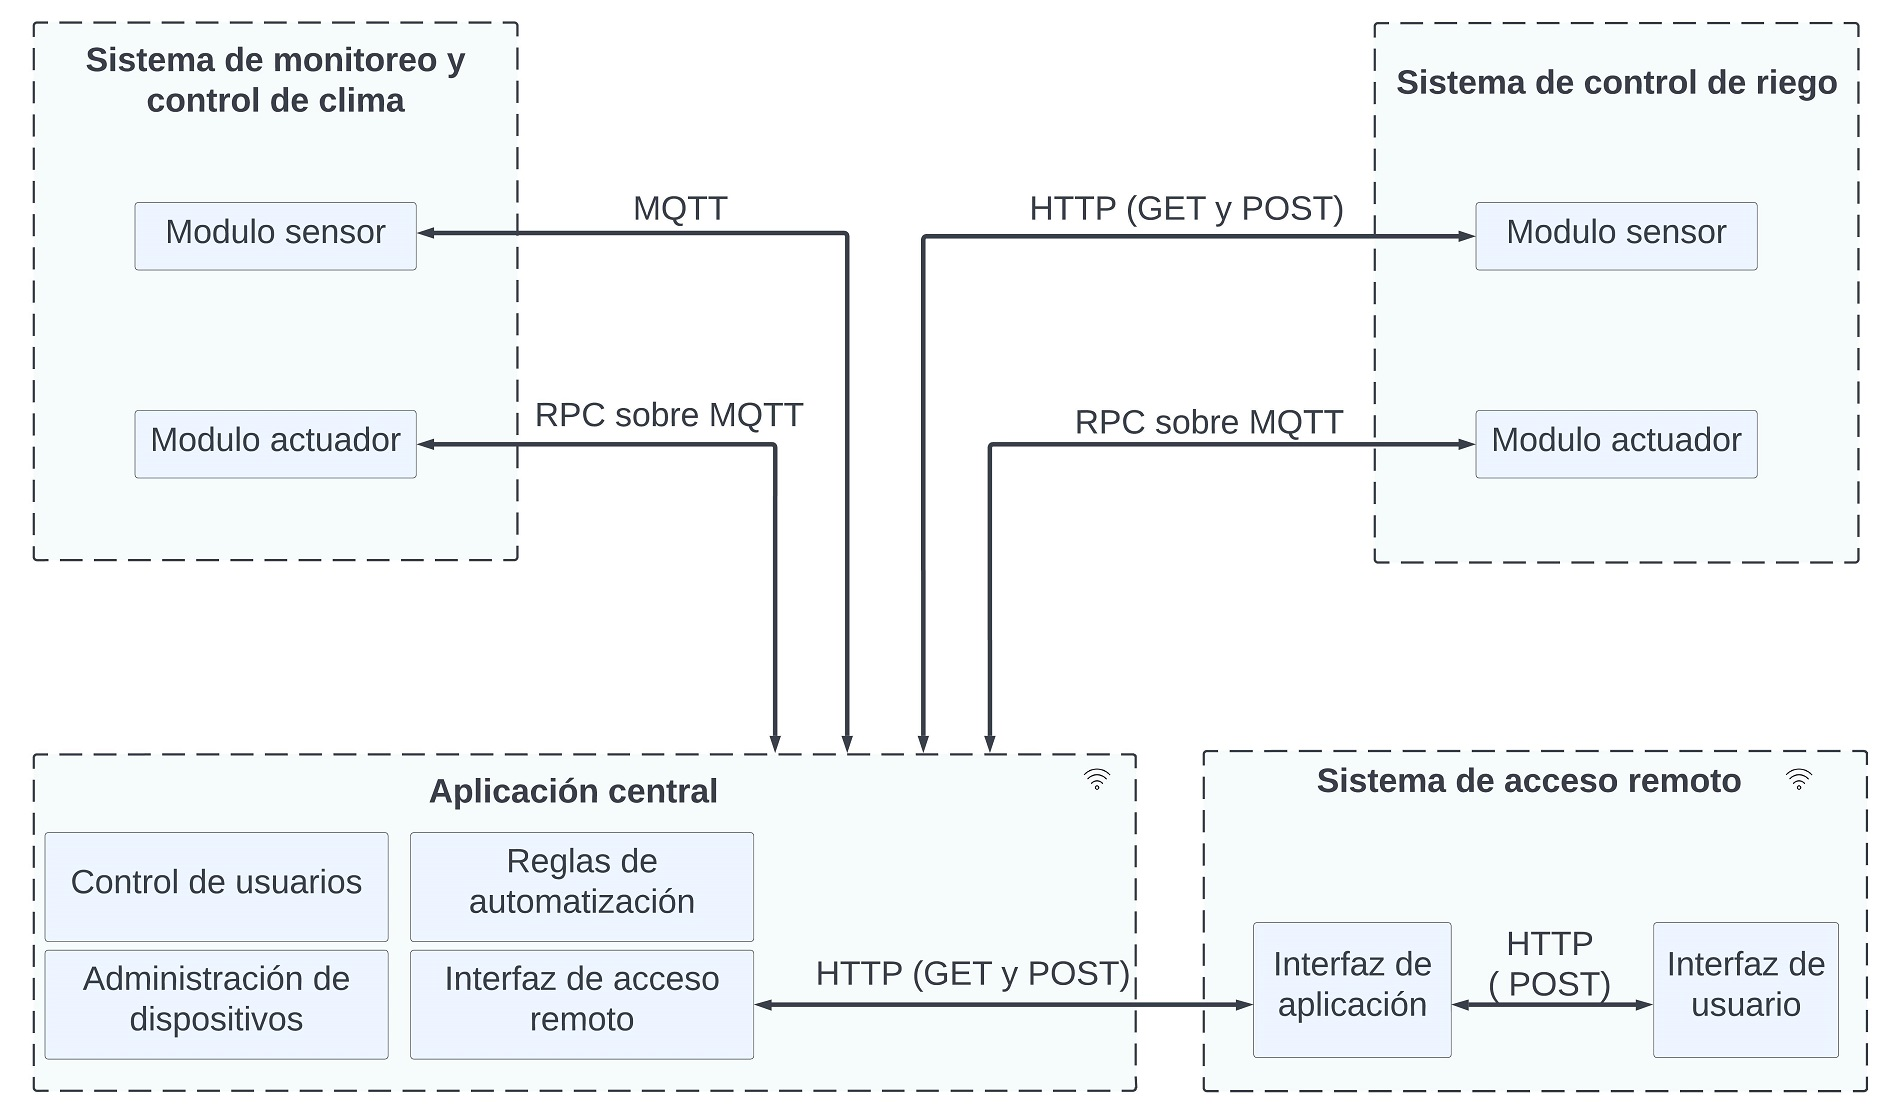
\includegraphics[width=1.0\textwidth]{./Figures/blockproto.jpg}
	\caption[Protocolos de comunicación entre módulos.]{Protocolos de comunicación entre módulos.}
	\label{fig:blockprotos}
\end{figure}

 A continuación se describen las comunicaciones principales entre sistemas:
 
 \begin{itemize}
	\item Sistema de monitoreo y control de clima: las comunicaciones desde y hasta este sistema son con la aplicación central.
	El módulo sensor envía las mediciones realizadas por medio de MQTT.
	En el caso que las variables del clima requieran una acción, la aplicación central comanda el encendido de los ventiladores por medio de un mensaje enviado por RPC sobre MQTT.
	
	\item Sistema de control de riego: las comunicaciones desde y hasta este sistemas son con la aplicación central.
	El módulo sensor realiza dos conexiones, una para el envío de las mediciones, y otra para recibir variables de configuración, como por ejemplo: el período de \textit{deep sleep}. Debido a limitaciones en la configuración de la persistencia de los mensajes en las colas de MQTT, se optó por utilizar llamadas HTTP POST y HTTP GET para realizar estas comunicaciones.
	Al igual que en el control de clima, la aplicación central iniciará el riego por medio de mensajes RCP sobre MQTT hacia el controlador de la bomba y de las válvulas.
	
	\item Sistema de acceso remoto: la interfaz se comunica con la aplicación por medio de pedidos de HTTP GET y POST para solicitar el reporte de estado de los diferentes componentes. Luego, estos son enviado hacia la interfaz de usuario por medio de un pedido HTTP POST.
 
 
 
 
 \end{itemize}






\section{Detalle de los módulos de hardware}
\label{sec:Módulos de hardware}

\subsection{Módulos sensores de humedad del suelo}
\label{Módulos sensores de humedad del suelo}

Estan compuestos por un ESP8266 y uno o dos sensores capacitivos de humedad del suelo lo que permite una mayor libertad a la hora de configurar los circuitos de riego.

\begin{figure}[!h]
	\centering
	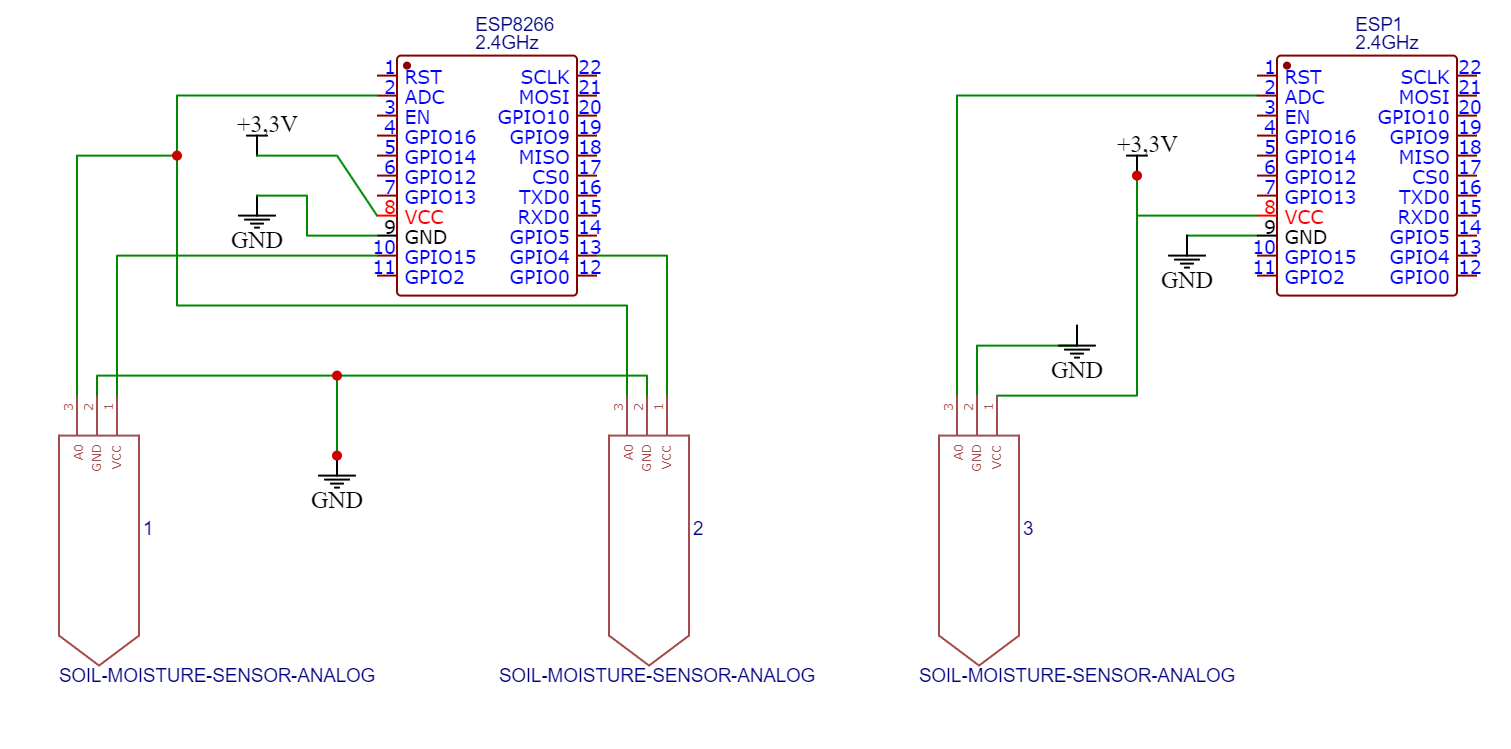
\includegraphics[width=0.9\textwidth]{./Figures/soil_schematic.png}
	\caption[Conexión del sensor de humedad del suelo]{Conexión del sensor de humedad del suelo.}
	\label{fig:soilschem}
\end{figure}


\begin{figure}[!htpb]
     \centering
     \begin{subfigure}[b]{0.45\textwidth}
		\centering
		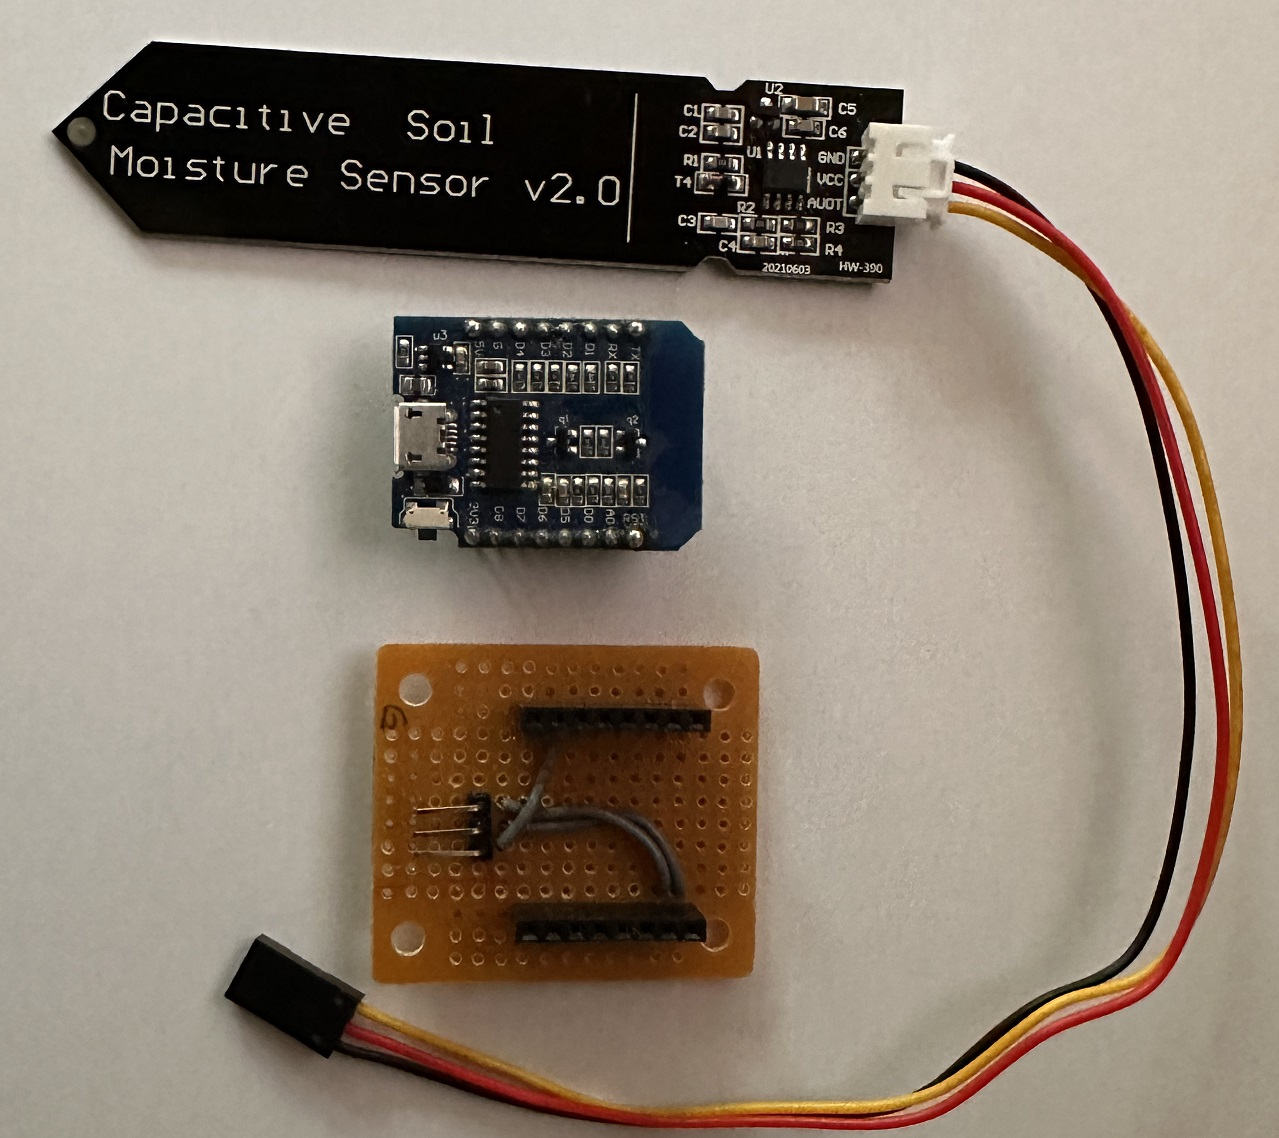
\includegraphics[width=0.60\textwidth]{./Figures/soil1.jpeg}
		\caption[Módulo con un sensor de humedad del suelo]{Módulo con un sensor de humedad del suelo.}
		\label{fig:soil1}
     \end{subfigure}
     \hfill
     \begin{subfigure}[b]{0.45\textwidth}
	\centering
		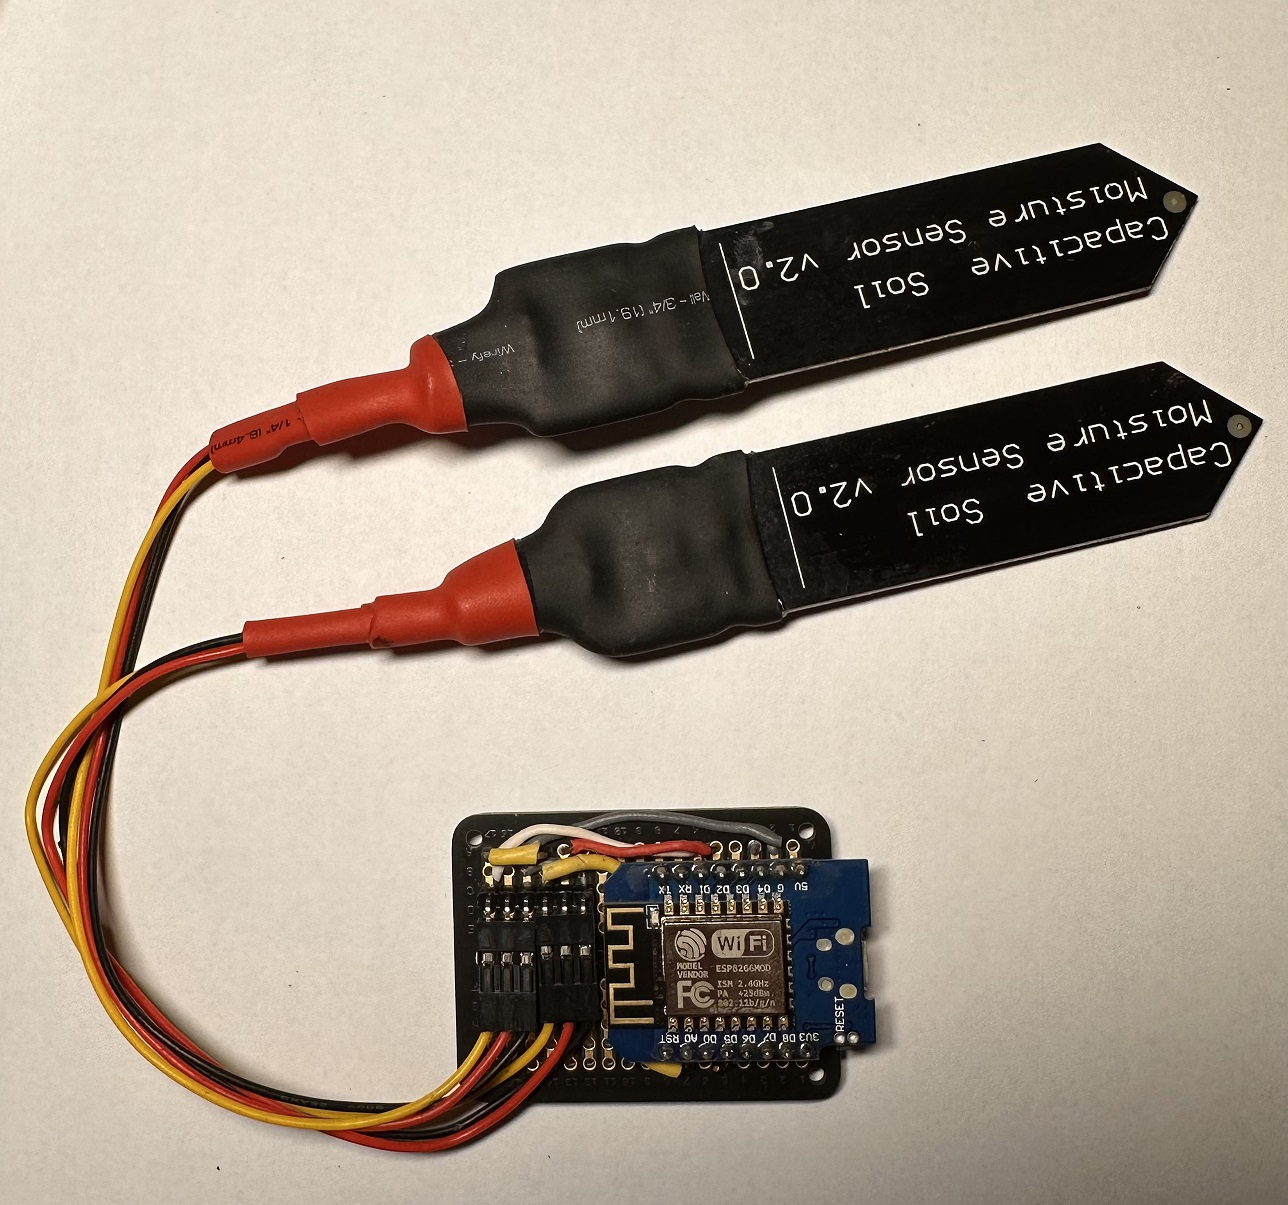
\includegraphics[width=0.60\textwidth]{./Figures/soil2.jpeg}
		\caption[Módulo con dos sensores de humedad del suelo]{Módulo con dos sensores de humedad del suelo.}
		\label{fig:soil2}
     \end{subfigure}
      \begin{subfigure}[b]{0.45\textwidth}
	\centering
		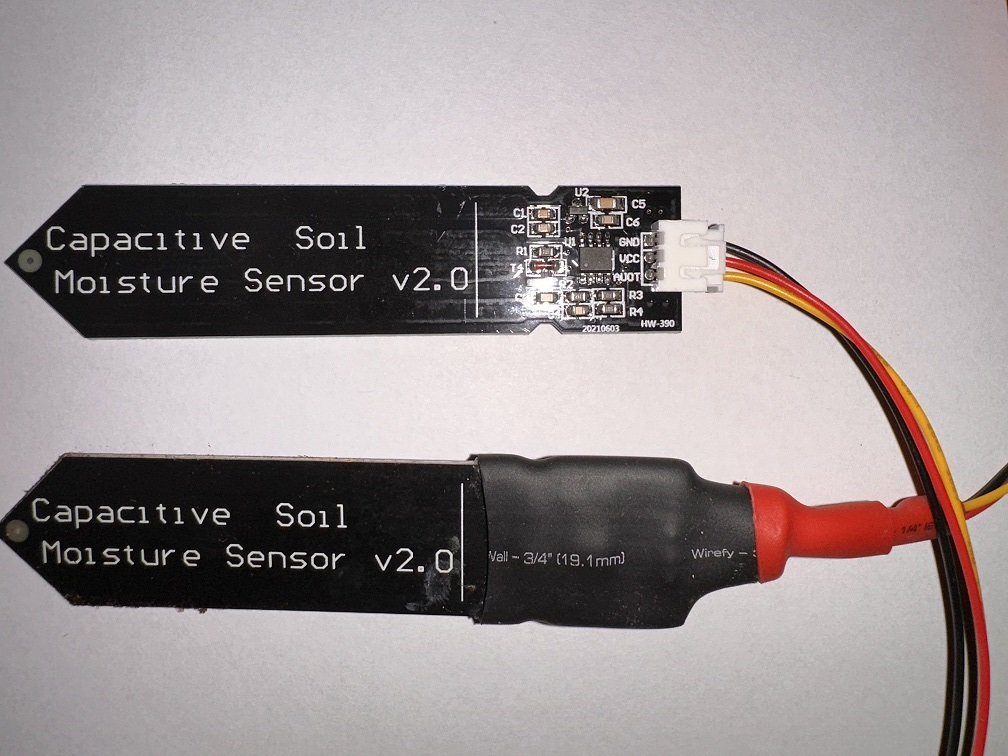
\includegraphics[width=0.60\textwidth]{./Figures/soil_compare.jpg}
		\caption[Detalle de protección de circuitos en los sensores]{Detalle de protección de circuitos en los sensores.}
     \end{subfigure}	
			\begin{subfigure}[b]{0.45\textwidth}
	\centering
		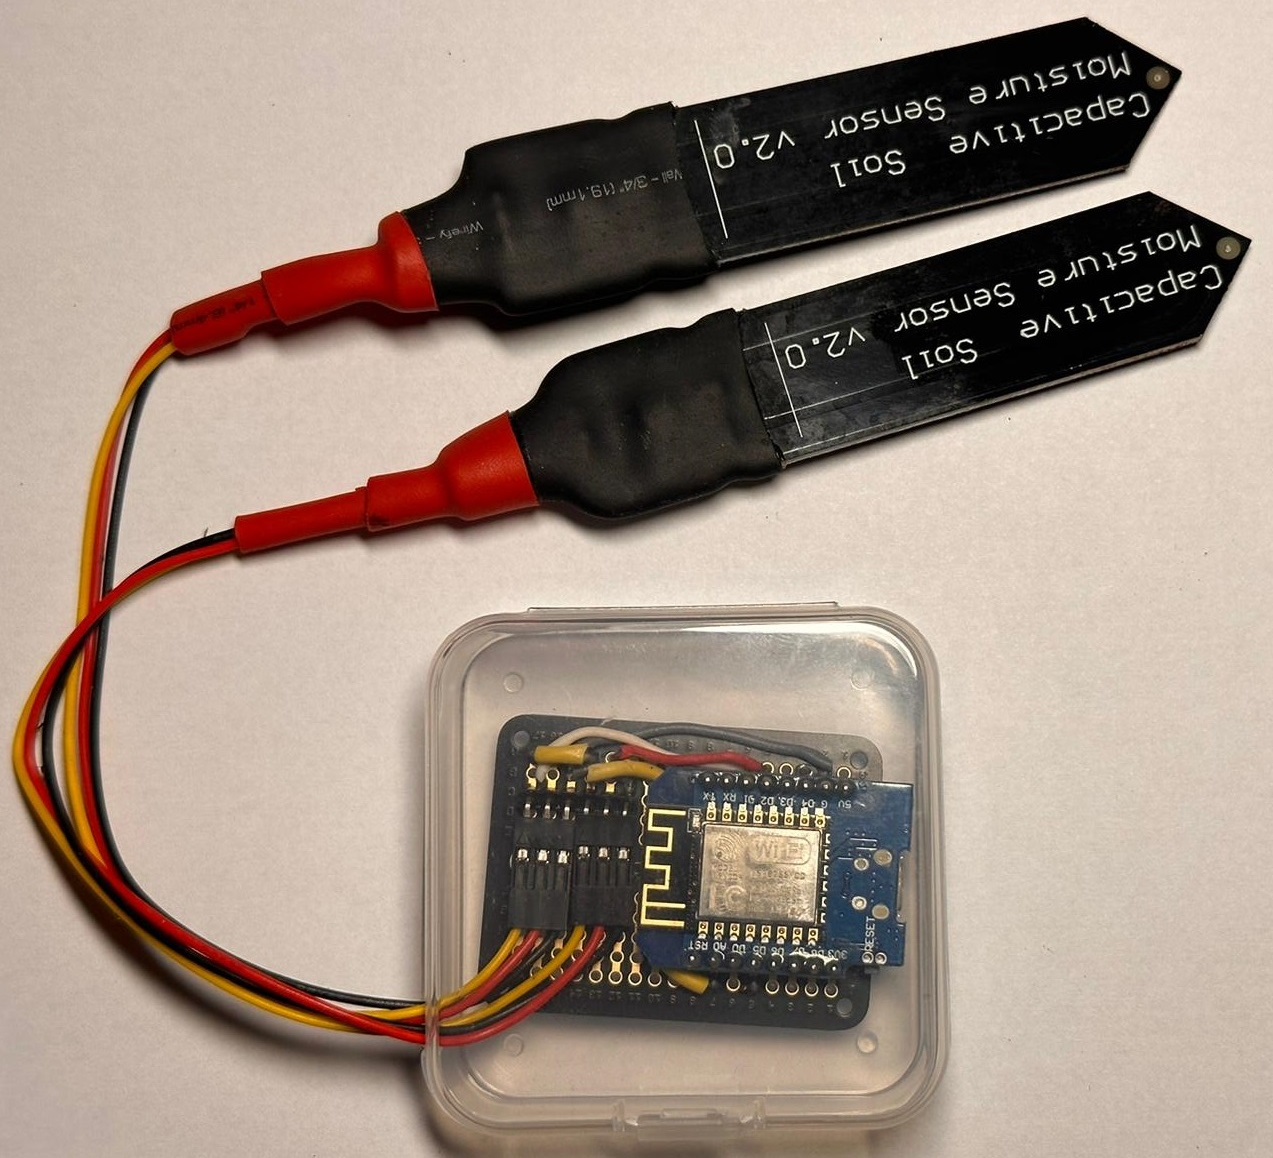
\includegraphics[width=0.60\textwidth]{./Figures/soil3.jpg}
		\caption[Módulo en su caja protectora]{Módulo en su caja protectora.}
		\label{fig:soil3}
     \end{subfigure}
     \hfill
        \caption[Módulos de sensores de humendad de suelo  empleados en el proyecto]{Módulo de sensores de humendad de suelo  empleados en el proyecto.}
        \label{fig:soilsenors}
\end{figure}



\subsection{Módulos controladores de riego}
\label{Módulos controladores de riego}

\begin{figure}[!h]
	\centering
	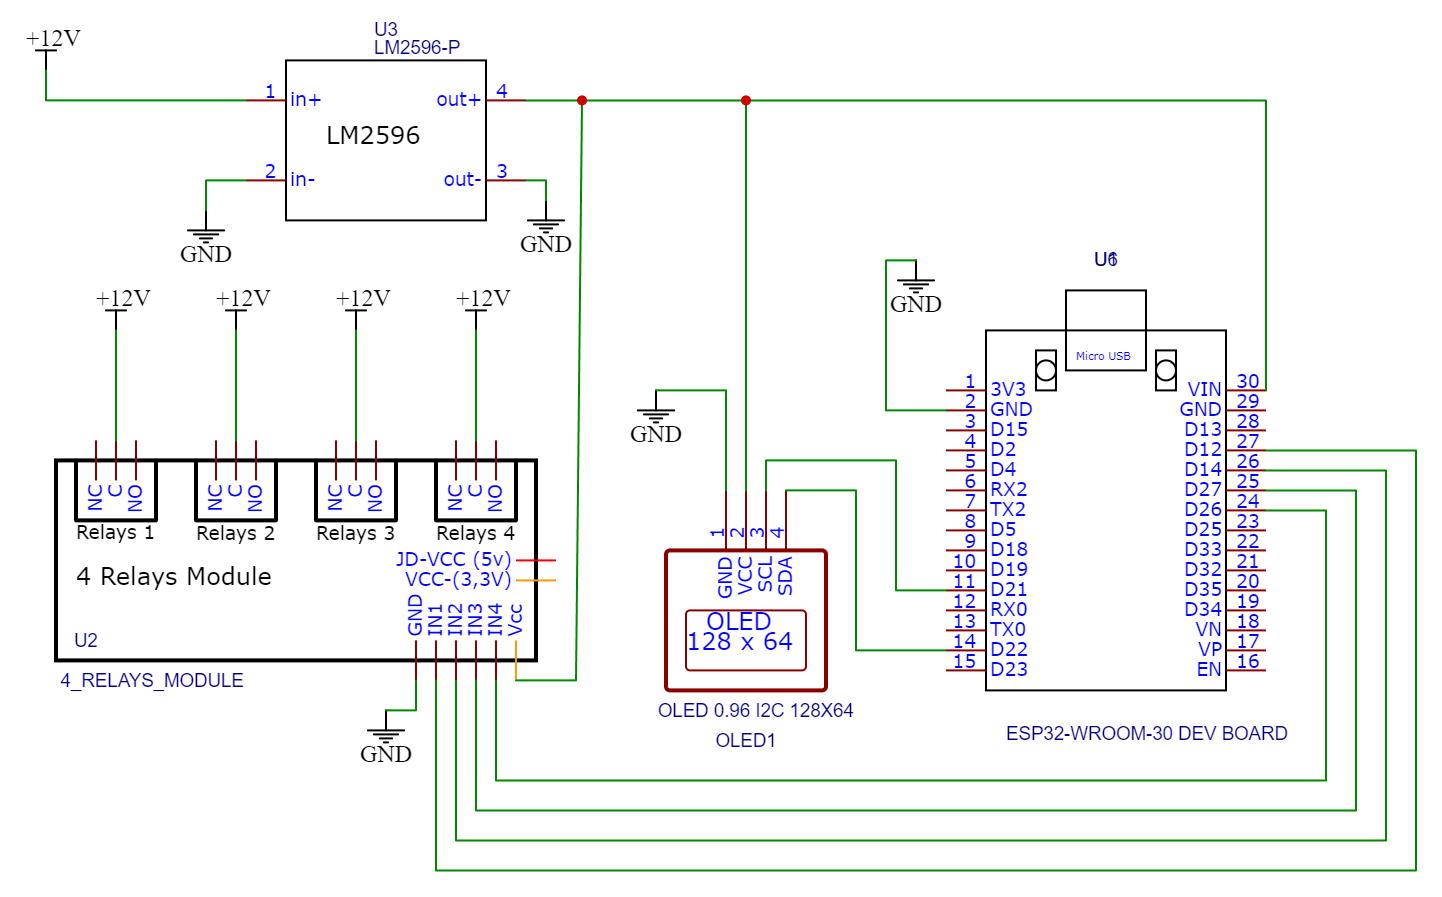
\includegraphics[width=0.9\textwidth]{./Figures/pump_schem.png}
	\caption[Conexión del modulo de control de riego]{Conexión del modulo de control de riego.}
	\label{fig:riegochem}
\end{figure}



\subsection{Módulos sensores de temperatura y humedad}
\label{Módulos sensores de temperatura y humedad}

\begin{figure}[!h]
	\centering
	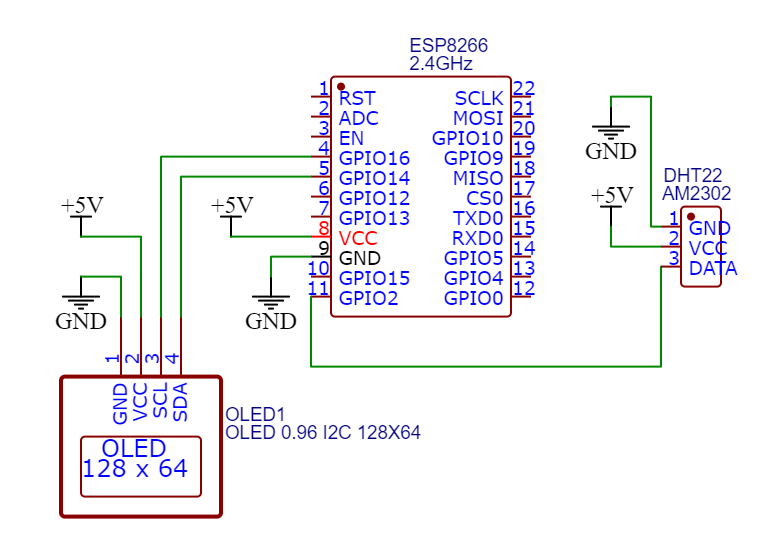
\includegraphics[width=0.7\textwidth]{./Figures/temp_sensor.png}
	\caption[Conexión del sensor de temperatura y humedad]{Conexión del sensor de temperatura y humedad
	.}
	\label{fig:tempschem}
\end{figure}


\begin{figure}[!h]
	\centering
	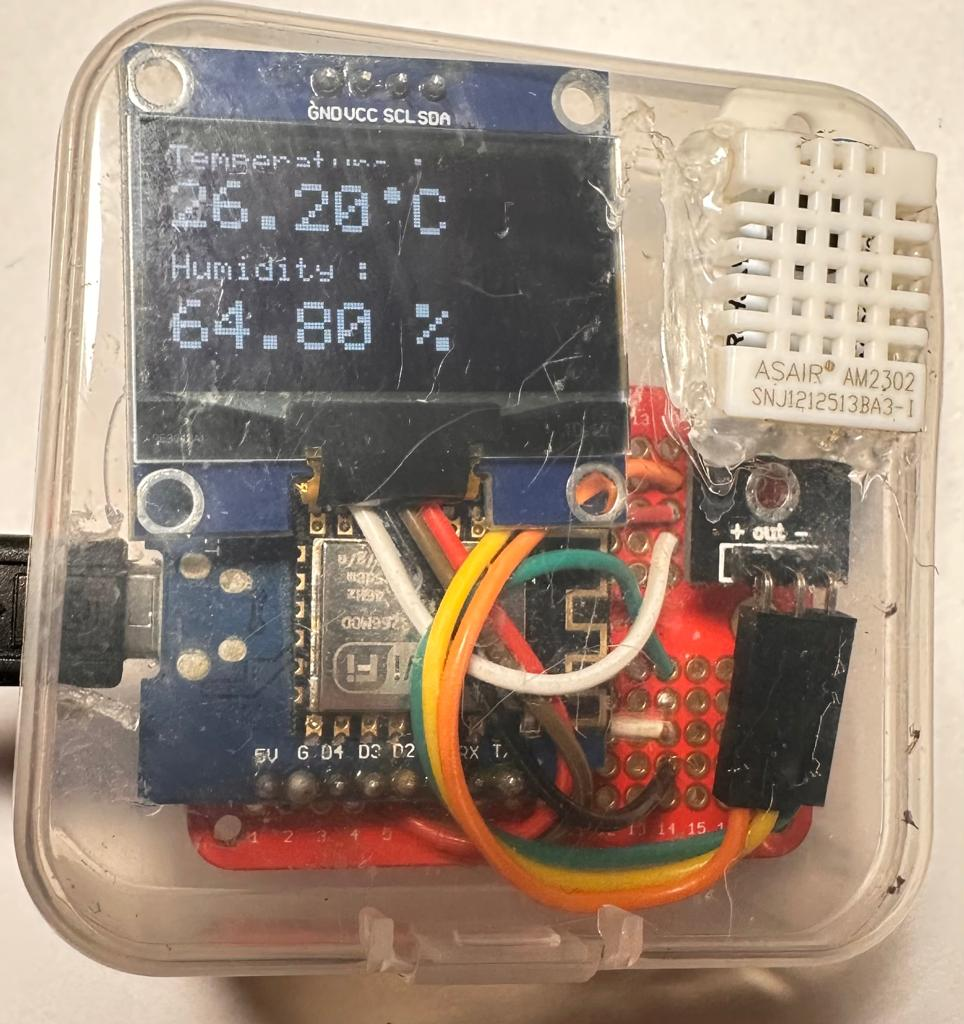
\includegraphics[width=0.5\textwidth]{./Figures/sensor_temp.jpg}
	\caption[Modulo completo en su caja protectora]{Modulo completo en su caja protectora.}
	\label{fig:temp_sensor}
\end{figure}

\subsection{Módulos controladores de clima}
\label{Módulos controladores de clima}

\begin{figure}[!h]
	\centering
	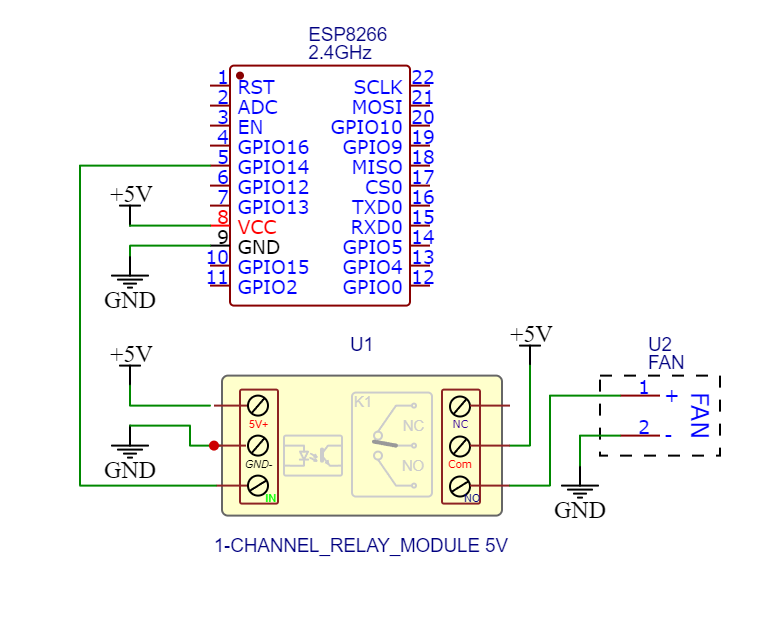
\includegraphics[width=0.7\textwidth]{./Figures/vent_schem.png}
	\caption[Conexión del modulo de control de clima]{Conexión del modulo de control de clima.}
	\label{fig:ventschem}
\end{figure}


\begin{figure}[!htpb]
     \centering
     \begin{subfigure}[b]{0.45\textwidth}
		\centering
		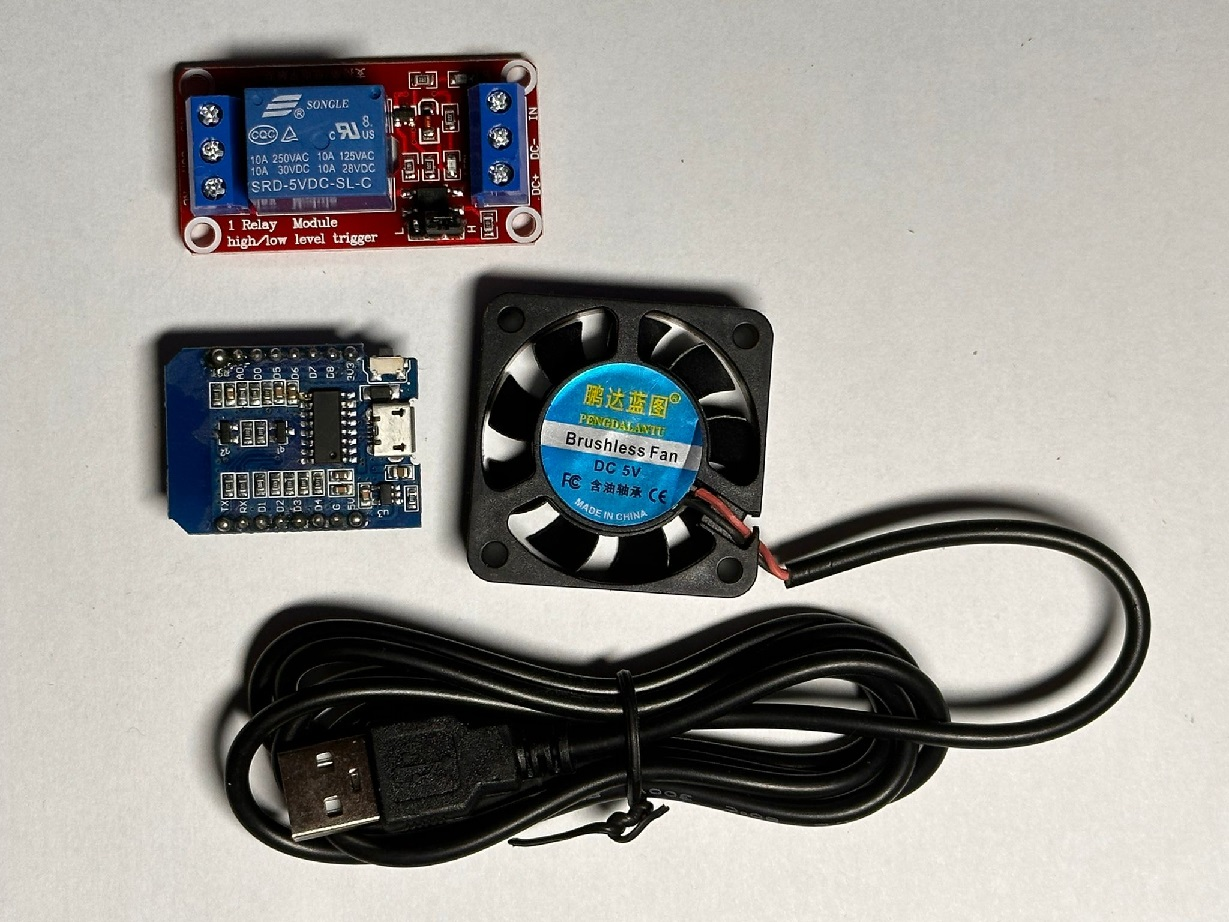
\includegraphics[width=0.80\textwidth]{./Figures/vent_control.jpg}
		\caption{Detalle de los componentes.}
		\label{fig:vent1}
     \end{subfigure}
     \hfill
     \begin{subfigure}[b]{0.45\textwidth}
	\centering
		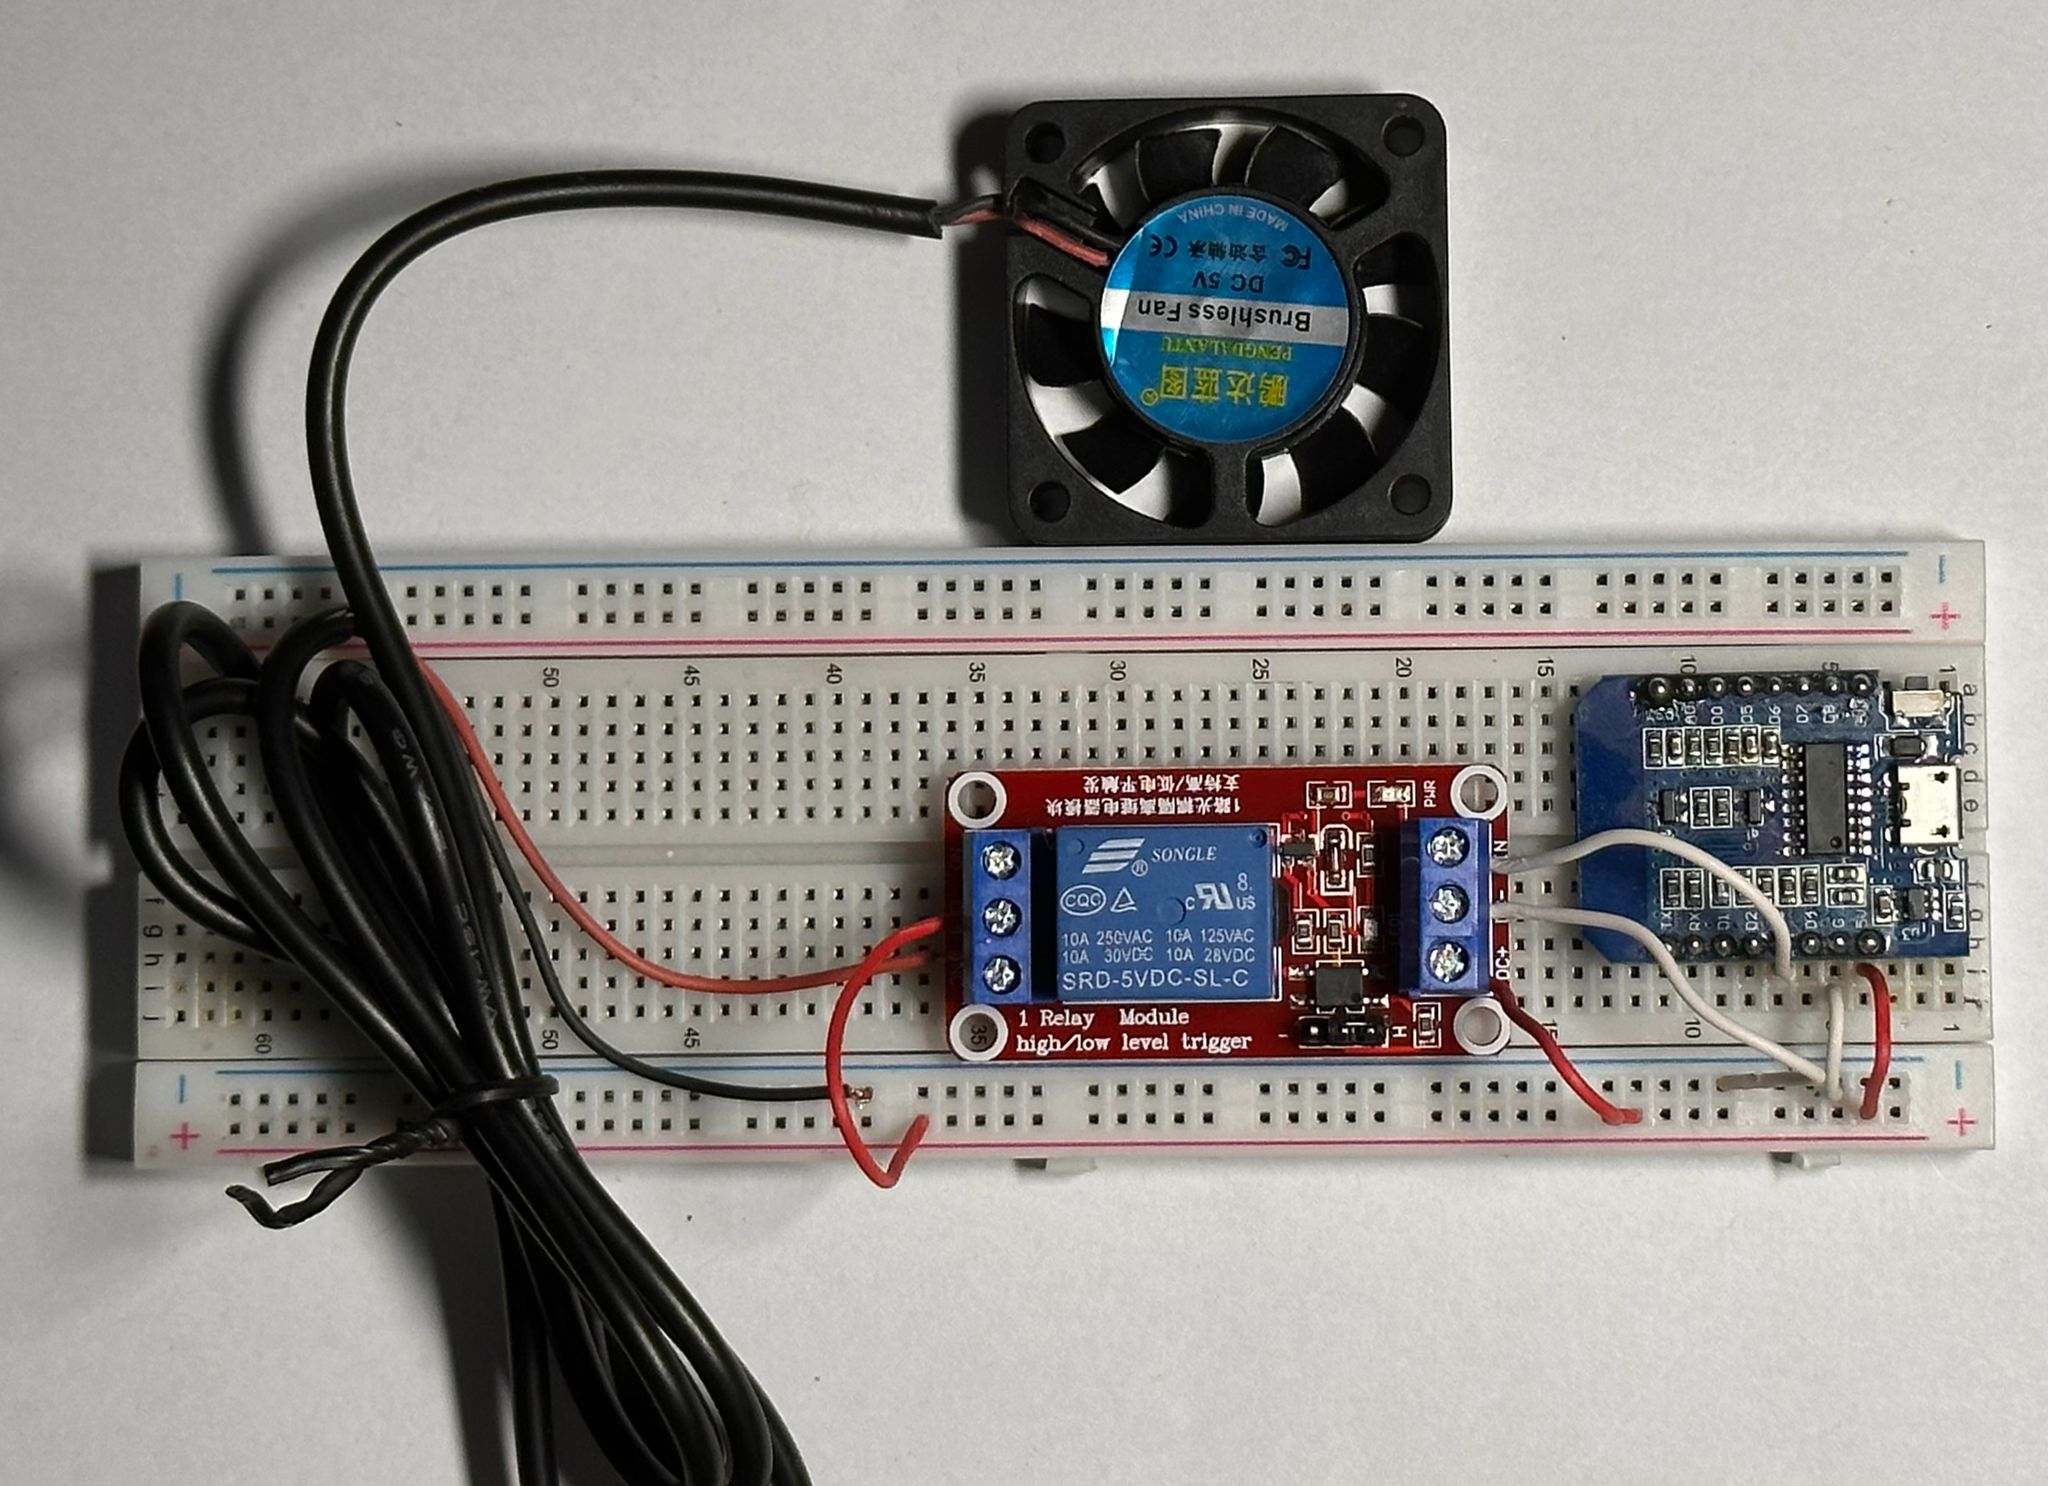
\includegraphics[width=0.80\textwidth]{./Figures/vent_proto.jpg}
		\caption{Configuración del módulo.}
		\label{fig:vent2}
     \end{subfigure}	
	\begin{subfigure}[b]{0.45\textwidth}
		\centering
		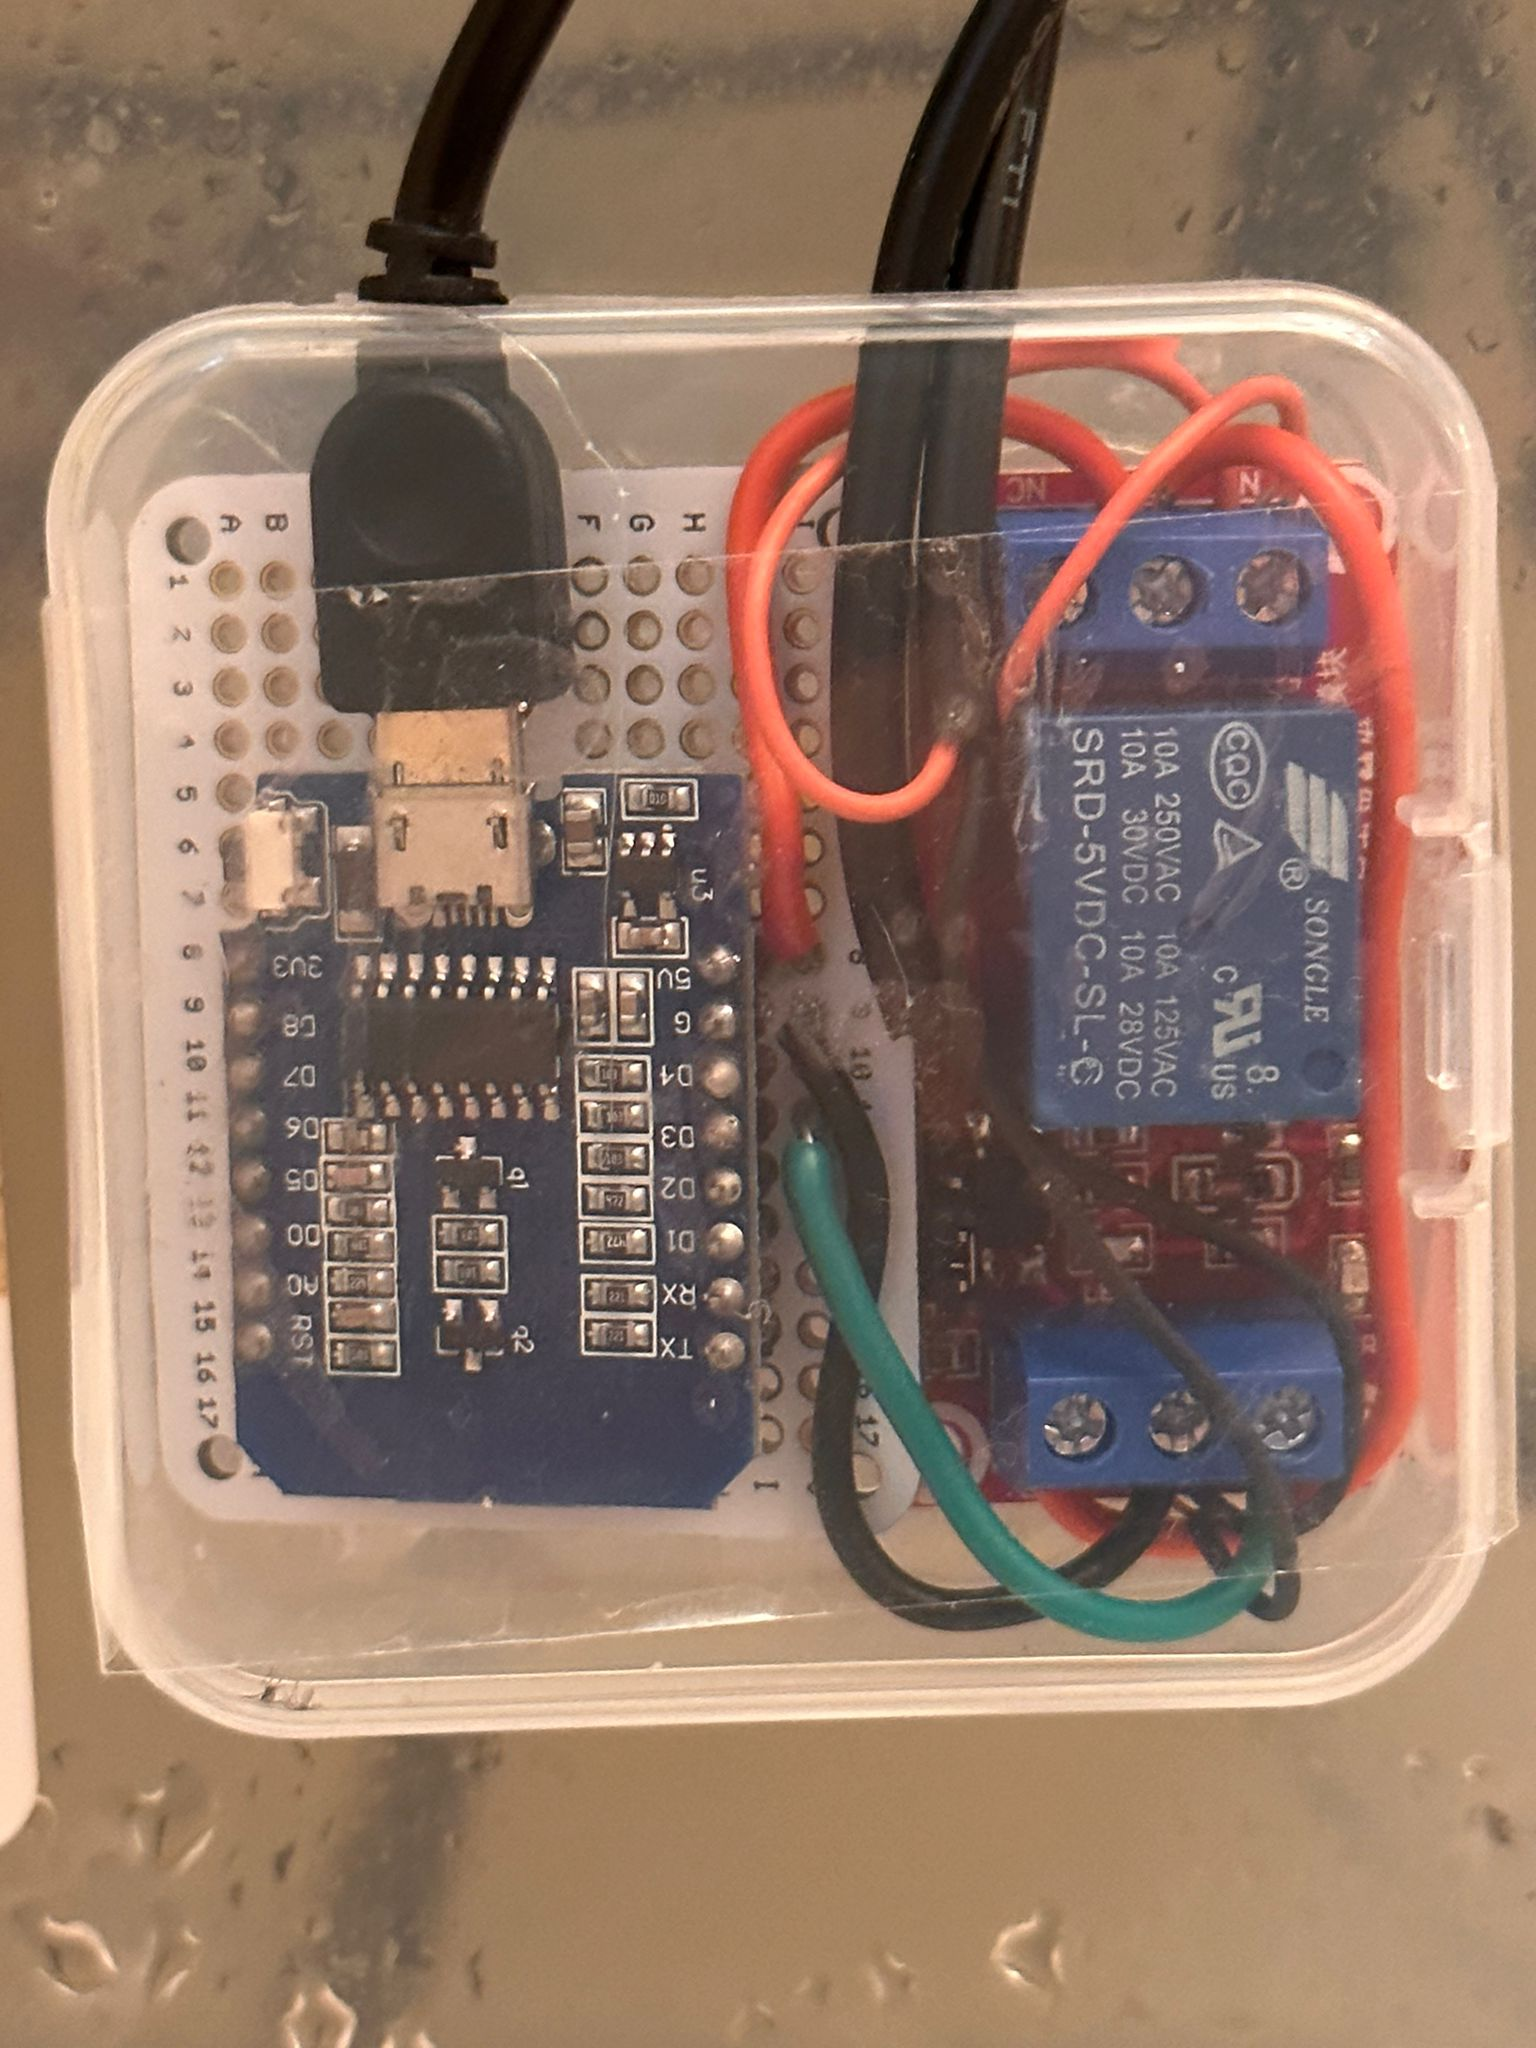
\includegraphics[width=0.60\textwidth]{./Figures/vent_assembled.jpg}
		\caption{Módulo finalizado en su caja protectora.}
		\label{fig:vent3}
     \end{subfigure}
     \hfill
        \caption[Módulo de control del clima]{Módulo de control del clima.}
        \label{fig:soilsenors}
\end{figure}




\section{Detalle del firmware desarrollado}
\label{sec:Desarrollo del firmware}


\subsection{Programación del microcontrolador de medición de clima}
\label{Programación del microcontrolador de medición de clima}

\section{Detalle del firmware desarrollado}
\label{sec:Desarrollo del firmware}


\section{Selección y configuración del software}
\label{sec:Selección y configuración del software}

\section{Ciberseguridad del sistema}
\label{sec:Ciberseguridad del sistema}
